\documentclass[12pt,a4paper]{article}
\usepackage[margin=22mm]{geometry}
\usepackage{fontspec}
\usepackage{xeCJK}
\usepackage{kotex}
\usepackage{graphicx}
\usepackage[table]{xcolor}
\usepackage{longtable}
\usepackage{booktabs}
\usepackage{array}
\usepackage{ragged2e}
\usepackage{enumitem}
\usepackage{hyperref}
\usepackage{amssymb}
\usepackage{fancyhdr}
\usepackage{titlesec}
\usepackage{setspace}
\usepackage{fvextra}
\setmainfont[Path=C:/Windows/Fonts/, BoldFont=malgunbd.ttf, ItalicFont=malgunsl.ttf]{malgun.ttf}
\setsansfont[Path=C:/Windows/Fonts/, BoldFont=malgunbd.ttf, ItalicFont=malgunsl.ttf]{malgun.ttf}
\setmonofont[Path=C:/Windows/Fonts/, BoldFont=malgunbd.ttf, ItalicFont=malgunsl.ttf]{malgun.ttf}
\newfontfamily\jpfont[Path=C:/Windows/Fonts/]{NotoSansJP-VF.ttf}
\setCJKmainfont[Path=C:/Windows/Fonts/, BoldFont=malgunbd.ttf, ItalicFont=malgunsl.ttf]{malgun.ttf}
\setCJKsansfont[Path=C:/Windows/Fonts/, BoldFont=malgunbd.ttf, ItalicFont=malgunsl.ttf]{malgun.ttf}
\setCJKmonofont[Path=C:/Windows/Fonts/]{malgun.ttf}
\XeTeXlinebreaklocale "ko"
\hyphenpenalty=10000
\exhyphenpenalty=10000
\binoppenalty=10000
\relpenalty=10000
\emergencystretch=2em
\sloppy
\newcommand{\DocNeedspace}[1]{\par\ifdim\dimexpr\pagegoal-\pagetotal\relax<#1\newpage\fi}
\providecommand{\tightlist}{\setlength{\itemsep}{0pt}\setlength{\parskip}{0pt}}
\newcommand{\SectionBreak}[2]{\texorpdfstring{#1\\[-0.10em]{\large #2}}{#1 #2}}
\newcommand{\SubsectionBreak}[2]{\texorpdfstring{#1\\[-0.10em]{\normalsize #2}}{#1 #2}}
\newcommand{\SubsubsectionBreak}[2]{\texorpdfstring{#1\\[-0.10em]{\normalsize #2}}{#1 #2}}
\providecommand{\pandocbounded}[1]{#1}
\RecustomVerbatimEnvironment{verbatim}{Verbatim}{breaklines=true,breakanywhere=true,fontsize=\scriptsize}
\hypersetup{colorlinks=true, linkcolor=black, urlcolor=blue}
\definecolor{DarkCharcoal}{HTML}{222222}
\definecolor{MainOrange}{HTML}{F26518}
\definecolor{MutedBrown}{HTML}{D44A14}
\definecolor{SoftBeige}{HTML}{FFF3E7}
\definecolor{CardPeach}{HTML}{FCE7DB}
\definecolor{SubTextGray}{HTML}{666666}
\definecolor{TableRule}{HTML}{B8A99D}
\color{DarkCharcoal}
\colorlet{LovvGreen}{MutedBrown}
\colorlet{LovvGreenDark}{DarkCharcoal}
\colorlet{LovvGold}{MainOrange}
\colorlet{LovvPaper}{SoftBeige}
\renewcommand{\arraystretch}{1.48}
\setlength{\tabcolsep}{3pt}
\setlength{\extrarowheight}{1pt}
\setlength{\LTpre}{6pt}
\setlength{\LTpost}{12pt}
\setlength{\LTleft}{0pt}
\setlength{\LTright}{0pt}
\arrayrulecolor{TableRule}
\newcolumntype{L}[1]{>{\RaggedRight\arraybackslash}m{#1}}
\newcolumntype{C}[1]{>{\centering\arraybackslash}m{#1}}
\newcommand{\TblHead}[2]{\multicolumn{1}{>{\centering\arraybackslash}m{#1}}{\textbf{#2}}}
\setlist[itemize]{leftmargin=*, itemsep=3pt, topsep=3pt}
\setlist[enumerate]{leftmargin=*, itemsep=3pt, topsep=3pt}
\setstretch{1.10}
\setlength{\parskip}{0.18\baselineskip}
\setlength{\headheight}{30pt}
\setcounter{tocdepth}{2}
\newcommand{\TocNoChildTight}{\vspace{-0.28em}}
\pagestyle{fancy}
\fancyhf{}
\lhead{\hbox{\makebox[42pt][c]{
\includegraphics[width=38pt,height=13pt,keepaspectratio]{../assets/images/SK-Networks-logo.png}}\hspace{0.7em}\makebox[42pt][c]{
\includegraphics[width=44pt,height=15pt,keepaspectratio]{../assets/images/en-core-logo.png}}\hspace{0.7em}\makebox[42pt][c]{
\includegraphics[width=38pt,height=13pt,keepaspectratio]{../assets/images/playdata-logo.png}}}}
\rhead{\scriptsize v1.0 | 실행 완료 | 로브 서비스 AgentCore 테스트 결과}
\cfoot{\thepage}
\renewcommand{\headrulewidth}{0.4pt}
\renewcommand{\headrule}{\hbox to\headwidth{\color{LovvGreen}\leaders\hrule height \headrulewidth\hfill}}
\begin{document}
\begin{titlepage}
\thispagestyle{empty}

\noindent \hbox to\textwidth{\makebox[0.28\textwidth][c]{
\includegraphics[width=0.22\textwidth,height=0.82cm,keepaspectratio]{../assets/images/SK-Networks-logo.png}}\hfil \makebox[0.28\textwidth][c]{
\includegraphics[width=0.26\textwidth,height=0.98cm,keepaspectratio]{../assets/images/en-core-logo.png}}\hfil \makebox[0.28\textwidth][c]{
\includegraphics[width=0.22\textwidth,height=0.82cm,keepaspectratio]{../assets/images/playdata-logo.png}}}
\vspace{1em}
\par\noindent\color{LovvGold}\rule{\textwidth}{1.2pt}\color{black}

\centering
\vspace*{0.16\textheight}
{\Huge\bfseries 테스트 결과 보고서\par}

\vspace{1.5em}
{\large 로브 서비스 AgentCore 테스트 결과\par}

\vfill
{\Large\bfseries 조라에몽의 만능 도구들\par}\vspace{0.8em}
{\Large 이창우, 전종혁, 조동휘, 최수아\\[0.8em]{\large 멘토 최민수}\par}
\vspace{2em}
{\large 2026-06-28\par}
\end{titlepage}
\begingroup
\fontsize{10.8pt}{12.2pt}\selectfont
\setlength{\parskip}{0pt}
\tableofcontents
\endgroup
\newpage


\newpage
\DocNeedspace{8\baselineskip}
\section*{1. 개요}
\addcontentsline{toc}{section}{1. 개요}

\DocNeedspace{24\baselineskip}
\begin{center}
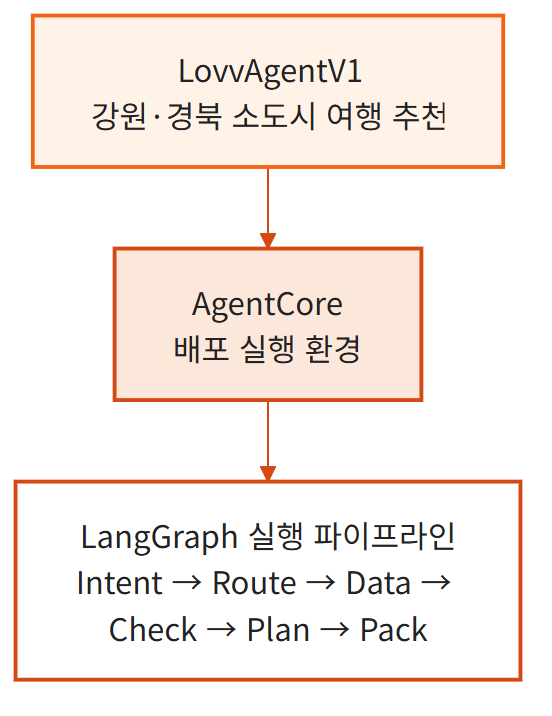
\includegraphics[width=0.86\linewidth,height=0.24\textheight,keepaspectratio]{../assets/images/mermaid/test-result-overview-01.png}
\par\vspace{0.3\baselineskip}
{\small LovvAgentV1 실행 구조\par}
\vspace{0.7\baselineskip}
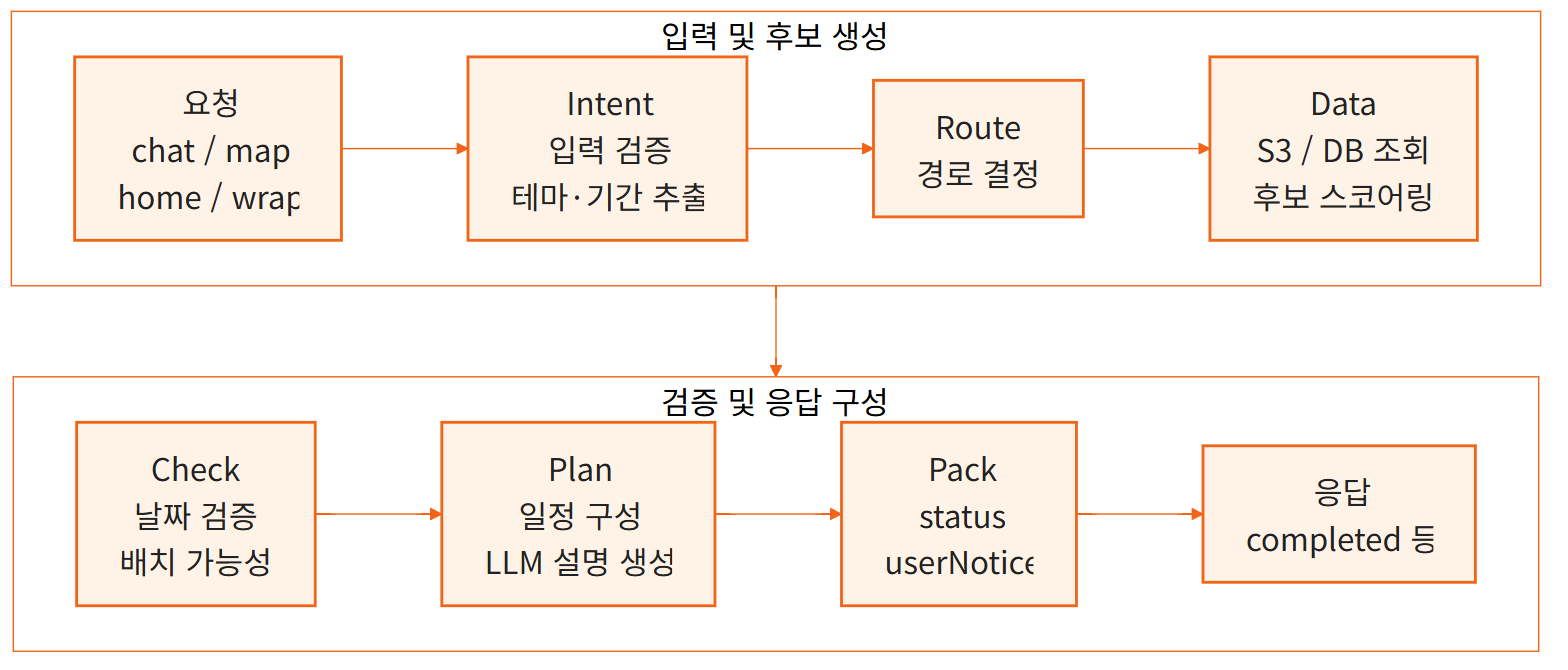
\includegraphics[width=0.98\linewidth,height=0.22\textheight,keepaspectratio]{../assets/images/mermaid/test-result-langgraph-pipeline-01.png}
\par\vspace{0.3\baselineskip}
{\small LangGraph 실행 Pipeline\par}
\vspace{0.7\baselineskip}
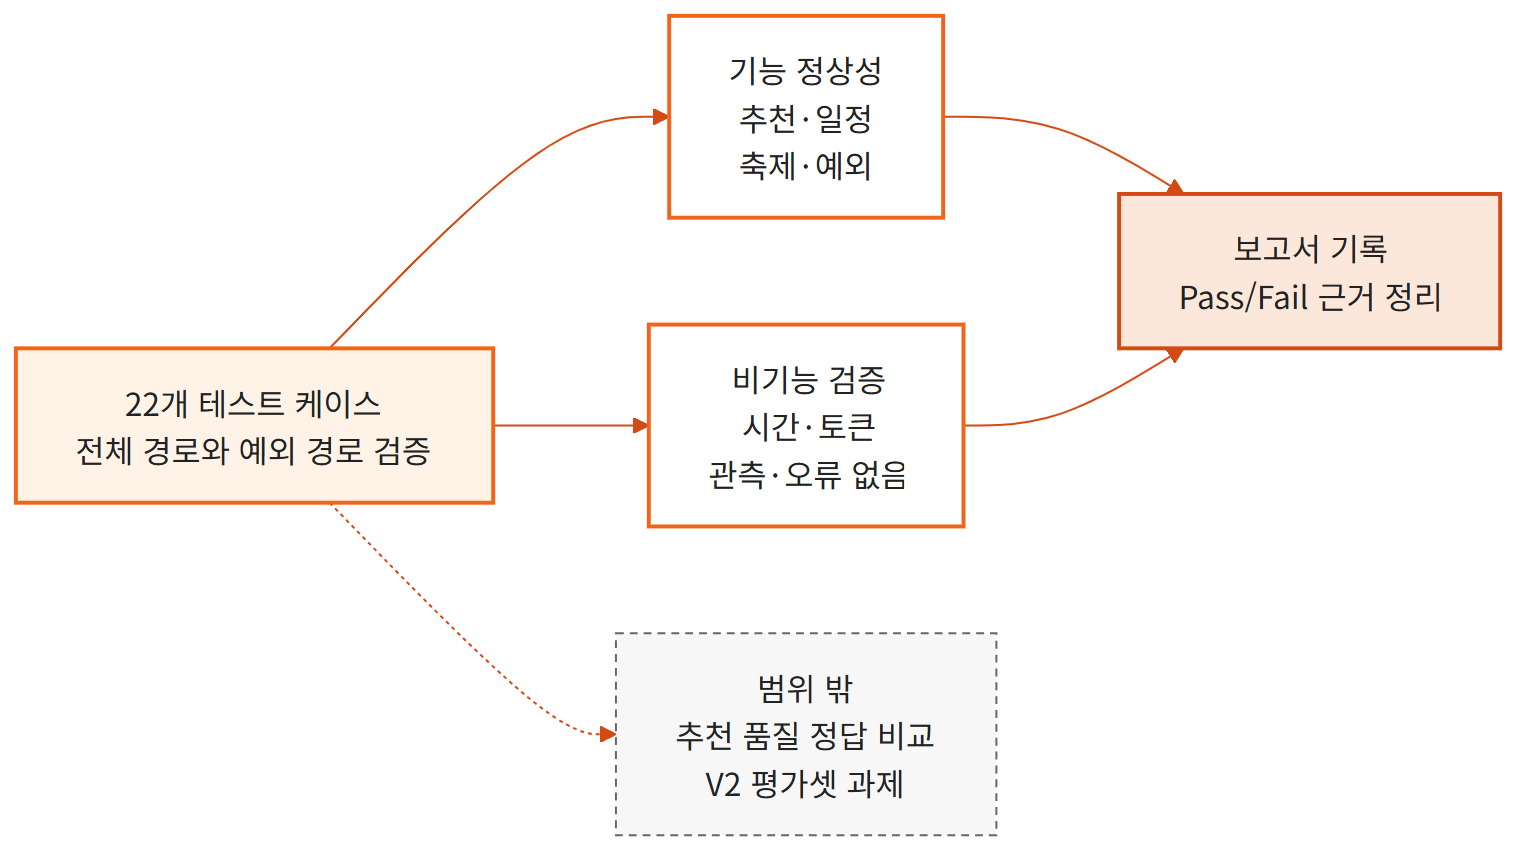
\includegraphics[width=0.92\linewidth,height=0.28\textheight,keepaspectratio]{../assets/images/mermaid/test-result-overview-02.png}
\par\vspace{0.3\baselineskip}
{\small LovvAgentV1 테스트 검증 범위\par}
\end{center}

\newpage
\DocNeedspace{18\baselineskip}
\subsection*{1.1 테스트 목적과 케이스 설계}
\addcontentsline{toc}{subsection}{1.1 테스트 목적과 케이스 설계}

\subsubsection*{1.1.1 목적}
\addcontentsline{toc}{subsubsection}{1.1.1 목적}

LovvAgentV1이 기능 요구사항 측면에서 설계된 추천·일정·축제·예외 처리 출력을 정상적으로 제공하는지 확인하고, 비기능 요구사항 측면에서 응답시간·토큰 사용량·관측 가능성을 충족하는지 검증한다.
\par\noindent 또한 배포 런타임의 \textbf{성능과 안정성}(무에러·잘못된 입력 격리·후보 부족 시 열화 동작)을 함께 확인한다.
\par\noindent 추천 "품질"의 정답 평가(어느 도시가 더 적합한가)는 별도 평가셋이 필요한 V2 과제로 본 범위 밖이다.

\subsubsection*{1.1.2 평가 범위}
\addcontentsline{toc}{subsubsection}{1.1.2 평가 범위}

본 테스트는 \textbf{추천 에이전트(LovvAgentV1)} 만 대상으로 한다.
\par\noindent 제품 요구사항은 프론트엔드·온보딩·지도 화면·북마크·개인화 등 더 넓은 기능을 포함하나, 그것들은 에이전트 밖이라 본 보고서 대상이 아니다.
\par\noindent 요구사항 정의가 비교적 개략적이므로, 각 케이스는 관련 요구사항(FR/NFR)에 \textbf{근사 매핑}했다.
\par\noindent 기능 요구사항 매핑은 4.1절 \textbf{요구사항} 표에서, 비기능 요구사항 매핑은 5.1절 \textbf{요구사항} 표에서 확인할 수 있다.

\textbf{케이스를 이렇게 세운 이유(왜 22개인가).}\quad "많이"가 아니라 \textbf{에이전트가 실제로 갈라지는 모든 경로를 한 번씩 덮는 최소 구성}을 목표로 했다.

\begin{itemize}
\tightlist
\item
  \textbf{진입 방식 3종}\par\noindent
  자연어 채팅 / 지도 마커(도시 고정) / 홈 추천.\par\noindent
  각 진입이 서로 다른 내부 경로를 타므로 모두 포함.\par\noindent
  (관련: FR-MAP-007 마커→일정유형→축제→추천)
\item
  \textbf{테마·기간 조합}\par\noindent
  단일·다중 테마 × 당일\textasciitilde{}2박3일.\par\noindent
  도시 선정과 일정 구성이 조합마다 달라지므로 대표 조합을 골고루 포함.\par\noindent
  (관련: FR-REC-001 입력 분류, FR-TRIP-001\textasciitilde004 일정 구성)
\item
  \textbf{축제 포함/미포함}\par\noindent
  축제 검증·배치 경로를 별도로 검증.\par\noindent
  (관련: FR-FES-001, FR-FEST-ENTRY-001)
\item
  \textbf{출발지 유무}\par\noindent
  출발지가 있으면 거리 반영 경로가 달라짐.
\item
  \textbf{예외·열화 경로}\par\noindent
  후보 부족(축소 일정)·불가능한 조합(추천 불가)·잘못된 입력(안전 거부).\par\noindent
  안정성과 폴백을 검증.\par\noindent
  (관련: NFR-005 폴백 제공)
\end{itemize}

\newpage
\DocNeedspace{18\baselineskip}
\subsection*{1.2 테스트 환경}
\addcontentsline{toc}{subsection}{1.2 테스트 환경}

\textbf{소프트웨어}

\begin{small}
\begin{longtable}{@{}L{0.205\linewidth}L{0.755\linewidth}@{}}
\toprule
\TblHead{0.205\linewidth}{항목} & \TblHead{0.755\linewidth}{값} \\
\midrule
\endhead
\bottomrule
\endlastfoot
런타임 & LovvAgentV1 (AWS Bedrock AgentCore Runtime) \\
런타임 ARN & \texttt{.\allowbreak{}.\allowbreak{}.\allowbreak{}:\allowbreak{}runtime/\allowbreak{}LovvAgentCore\_\allowbreak{}LovvAgentV1-\allowbreak{}PumZyEGRsT} \\
리전 / Python & us-east-1 / 3.12 \\
프레임워크 & LangGraph (상태 그래프 파이프라인) \\
LLM & \texttt{openai.\allowbreak{}gpt-\allowbreak{}oss-\allowbreak{}120b-\allowbreak{}1:\allowbreak{}0} (전 노드 공통, \texttt{reasoning\_\allowbreak{}effort="low"}) \\
Embedding & \texttt{amazon.\allowbreak{}titan-\allowbreak{}embed-\allowbreak{}text-\allowbreak{}v2:\allowbreak{}0} \\
벡터 저장소 & S3 Vectors: \texttt{lovv-\allowbreak{}agentcore-\allowbreak{}v1-\allowbreak{}vector} / \texttt{kr-\allowbreak{}agentcore-\allowbreak{}v1} \\
DB & Dynamo\allowbreak{}DB: \texttt{TourKoreaDomainData} \\
Observability & OTel → ADOT Collector → X-Ray + CloudWatch \\
\end{longtable}
\end{small}

\textbf{하드웨어 / 인프라}

\begin{small}
\begin{longtable}{@{}L{0.205\linewidth}L{0.755\linewidth}@{}}
\toprule
\TblHead{0.205\linewidth}{항목} & \TblHead{0.755\linewidth}{값} \\
\midrule
\endhead
\bottomrule
\endlastfoot
배포 런타임 & AWS Bedrock AgentCore: \textbf{관리형 서버리스}(호출마다 격리된 실행 인스턴스 생성) / CPU·메모리는 AWS가 관리하며 사양 비공개 \\
런타임 구성 & Python 3.12, 공개 엔드포인트, 연결/읽기 타임아웃 60초 \\
세션 모드 & 본 테스트는 호출마다 새 인스턴스 = \textbf{콜드 시작}(요청 간 완전 격리) / 워밍 재사용은 사용하지 않음 \\
네트워크 & us-east-1 리전, 공개 엔드포인트 \\
\end{longtable}
\end{small}

\DocNeedspace{6\baselineskip}
\subsection*{1.3 용어 안내 (약식)}
\addcontentsline{toc}{subsection}{1.3 용어 안내 (약식)}

평가자가 본문을 읽을 때 참고할 최소 용어다.

\begin{itemize}
\tightlist
\item
  \textbf{파이프라인 단계(노드):} 의도 분석 → 단계 라우팅 → 후보 도시·장소 검색 → 축제 검증 → 일정 구성 → 응답 정리.\par\noindent
  (코드명: intent → supervisor → candidate\_evidence → festival\_verifier → planner → response\_packager)
\item
  \textbf{출력 상태값:} \texttt{ok}=정상 추천 / \texttt{insufficient}=후보 부족으로 축소 일정 / \texttt{no\_\allowbreak{}candidate}=추천 불가(재질의) / \texttt{END\_\allowbreak{}WAIT\_\allowbreak{}USER}=사용자 재입력 대기.
\item
  \textbf{\texttt{no\_\allowbreak{}city\_\allowbreak{}after\_\allowbreak{}theme\_\allowbreak{}gate}:} 요청 테마를 만족하는 도시가 하나도 없음(추천 불가 사유).
\item
  \textbf{콜드 시작:} 요청마다 새 인스턴스를 띄우는 격리 실행(워밍 재사용보다 느림).
\end{itemize}

\newpage
\DocNeedspace{8\baselineskip}
\section*{\SectionBreak{2. 테스트 전략}{2-Path}}
\addcontentsline{toc}{section}{2. 테스트 전략 / 2-Path}

기능과 비기능은 \textbf{수집원이 다르다.}
\par\noindent 두 경로는 상호 보완이며 어느 하나로 전부를 대체할 수 없다.

\begin{small}
\begin{longtable}{@{}L{0.195\linewidth}L{0.355\linewidth}L{0.405\linewidth}@{}}
\toprule
\TblHead{0.195\linewidth}{} & \multicolumn{1}{>{\centering\arraybackslash}m{0.355\linewidth}}{\textbf{Path 1}\par\noindent 로컬 e2e} & \multicolumn{1}{>{\centering\arraybackslash}m{0.405\linewidth}}{\textbf{Path 2}\par\noindent 배포 텔레메트리} \\
\midrule
\endhead
\bottomrule
\endlastfoot
도구 & \texttt{capture\_\allowbreak{}e2e\_\allowbreak{}state.\allowbreak{}py\ -\allowbreak{}\/\allowbreak{}-\allowbreak{}live} & \texttt{invoke\_\allowbreak{}deployed\_\allowbreak{}runtime.\allowbreak{}py} → \texttt{fetch\_\allowbreak{}traces.\allowbreak{}py} \\
실행 & src 인-프로세스 (로컬) & 배포 클라우드 런타임 \\
산출물 & \texttt{e2e\_\allowbreak{}state\_\allowbreak{}dump\_\allowbreak{}*.\allowbreak{}json} (노드 내부 state) & X-Ray segment + \texttt{AGENT\_\allowbreak{}NODE\_\allowbreak{}METRIC} 로그 \\
\textbf{담는 것} & 추천 내용 (도시·status·축제·일정), 노드 방문 순서 & 서비스 콜 시간, 노드별 시간/토큰, 무에러 여부 \\
\textbf{못 담는 것} & 실행시간 (로컬값, 비대표) & 추천 내용 (마스킹/변환으로 소실) \\
용도 & \textbf{기능 검증 (4장 기능 테스트)} & \textbf{비기능 검증 (5장 비기능 테스트)} \\
\end{longtable}
\end{small}

\begin{quote}
배포 런타임의 공개 응답·텔레메트리에는 마스킹 전 노드 state가 없다.
\par\noindent 따라서 "어느 도시를 골랐고 무엇을 만들었는가"는 Path 1로만 증빙된다.
\par\noindent 반대로 프로덕션 실행시간·X-Ray 관측은 Path 2로만 측정된다.
\end{quote}


\newpage
\DocNeedspace{8\baselineskip}
\section*{3. 실행 절차 \& 화면}
\addcontentsline{toc}{section}{3. 실행 절차 \& 화면}

\DocNeedspace{6\baselineskip}
\subsection*{3.1 실행 명령}
\addcontentsline{toc}{subsection}{3.1 실행 명령}

\begin{verbatim}
# Path 1
# 로컬 기능 캡처 (e2e state dump)
$env:LOVV_ENABLE_AWS_SMOKE='1'
uv run scripts/capture_e2e_state.py --live --input-dir docs/tasks/results/test_cases
# → docs/tasks/results/test_cases/results/e2e_state_dump_<NN>_<name>_<timestamp>.json (케이스당 1개)

# Path 2
# 배포 invoke 후 트레이스/로그 수집
uv run scripts/invoke_deployed_runtime.py --input-dir docs/tasks/results/test_cases
uv run scripts/fetch_traces.py --since-min 90 --profile skn26_final           # 최근 트레이스 id 목록
uv run scripts/fetch_traces.py --summary docs/tasks/results/deployed_trace_ids.json \
    --out docs/tasks/results/traces_fetched.json --raw --logs --profile skn26_final
\end{verbatim}

\DocNeedspace{6\baselineskip}
\subsection*{\SubsectionBreak{3.2 AWS 콘솔}{트레이스 확인 화면 (CloudWatch GenAI Observability / X-Ray)}}
\addcontentsline{toc}{subsection}{3.2 AWS 콘솔 / 트레이스 확인 화면 (CloudWatch GenAI Observability / X-Ray)}

아래 3장은 \textbf{같은 한 요청}(POST /invocations, 총 11.11s)의 콘솔 캡처다.
\par\noindent 화면 1은 호출 구조(trace map), 화면 2·3은 같은 trace timeline의 상단·하단이다.
\par\noindent 이 절은 별도 콘솔 접속 없이 \textbf{현재 PDF와 포함된 PNG 캡처만으로} 무엇을 확인해야 하는지 알 수 있도록, 사진별 파일명·판독 포인트·문서 내 참고 위치를 함께 적는다.

\DocNeedspace{18\baselineskip}
\begin{small}
\begin{longtable}{@{}L{0.145\linewidth}L{0.230\linewidth}L{0.380\linewidth}L{0.180\linewidth}@{}}
\toprule
\TblHead{0.145\linewidth}{화면} & \TblHead{0.230\linewidth}{현재 파일} & \TblHead{0.380\linewidth}{확인 가능한 정보} & \TblHead{0.180\linewidth}{문서 내 참고 위치} \\
\midrule
\endhead
\bottomrule
\endlastfoot
화면 1 & \texttt{observability\_\allowbreak{}1.png} & 요청 → LangGraph → 노드 → 서비스 서브콜의 전체 호출 구조 & 5장 서비스 지연, 9장 구조적 한계 \\
화면 2 & \texttt{observability\_\allowbreak{}2.png} & intent·candidate\_evidence 구간의 LLM 시간, S3 Vectors 4회, DynamoDB BatchGetItem 1회 & 5.2절 서비스 콜 지연 \\
화면 3 & \texttt{observability\_\allowbreak{}3.png} & planner 구간의 DynamoDB GetItem 5회와 BedrockConverse 병목 & 9.2절 L2/L3 보완 지점 \\
\end{longtable}
\end{small}

\DocNeedspace{44\baselineskip}
\phantomsection
\subsubsection*{\SubsubsectionBreak{3.2.1 화면 1}{Trace map}}
\addcontentsline{toc}{subsubsection}{3.2.1 화면 1 / Trace map}

\textbf{확인 포인트}
\begin{RaggedRight}
\begin{itemize}
\item \textbf{흐름:} LovvAgentInvocation → invoke\_agent LangGraph → 노드 실행 순서로 이어진다.
\item \textbf{노드:} intent, supervisor, candidate\_evidence, planner, response\_packager가 표시된다.
\item \textbf{서브콜:} S3Vectors.QueryVectors, DynamoDB.BatchGetItem/GetItem, BedrockConverse 호출 구조를 확인할 수 있다.
\item \textbf{해석:} 이 화면은 파이프라인 구조와 각 노드의 외부 서비스 호출을 확인하는 근거다.
\end{itemize}
\end{RaggedRight}

\begin{center}
\pandocbounded{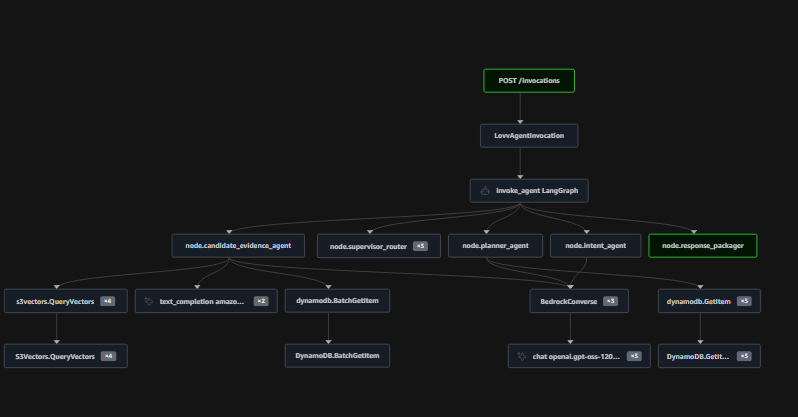
\includegraphics[width=0.95\linewidth,height=0.60\textheight,keepaspectratio]{../assets/images/agentcore_v1_observability/observability_1.png}}
\end{center}

\DocNeedspace{44\baselineskip}
\phantomsection
\subsubsection*{\SubsubsectionBreak{3.2.2 화면 2}{Trace 상세 타임라인 상단}}
\addcontentsline{toc}{subsubsection}{3.2.2 화면 2 / Trace 상세 타임라인 상단}

\textbf{확인 포인트}
\begin{RaggedRight}
\begin{itemize}
\item \textbf{구간:} intent → candidate\_evidence.
\item \textbf{LLM:} intent\_agent 2.45s, candidate\_evidence\_agent 내부 BedrockConverse 3.56s.
\item \textbf{검색/DB:} S3Vectors.QueryVectors ×4 = 0.36s, DynamoDB.BatchGetItem = 0.04s.
\item \textbf{해석:} 검색·DB는 1초 미만이며, 지연은 주로 LLM 호출에 집중된다.
\end{itemize}
\end{RaggedRight}

\begin{center}
\pandocbounded{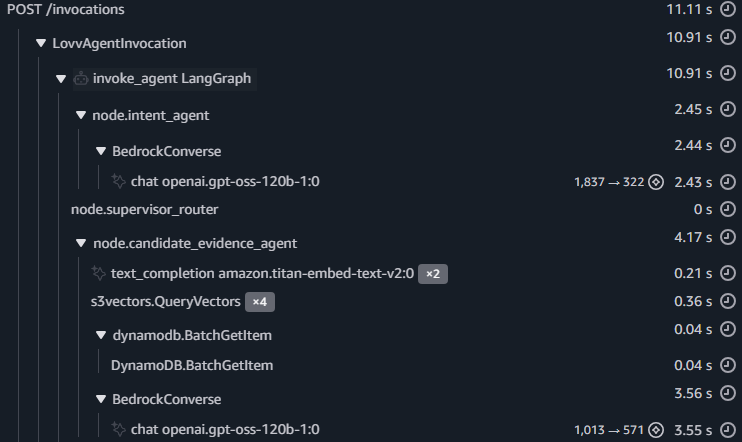
\includegraphics[width=0.95\linewidth,height=0.60\textheight,keepaspectratio]{../assets/images/agentcore_v1_observability/observability_2.png}}
\end{center}

\DocNeedspace{44\baselineskip}
\phantomsection
\subsubsection*{\SubsubsectionBreak{3.2.3 화면 3}{같은 타임라인 하단}}
\addcontentsline{toc}{subsubsection}{3.2.3 화면 3 / 같은 타임라인 하단}

\textbf{확인 포인트}
\begin{RaggedRight}
\begin{itemize}
\item \textbf{구간:} planner → packager.
\item \textbf{DB:} DynamoDB.GetItem ×5 = 0.03s.
장소별 개별 조회 구조라 9.2절 L2의 N+1 보완 근거가 된다.
\item \textbf{LLM:} BedrockConverse 4.25s(3837→953 tok).
일정 설명 생성 구간의 단일 최대 병목이다.
\item \textbf{해석:} supervisor\_router·response\_packager는 0s이고, 병목은 planner 내부 LLM 호출에 집중된다.
\end{itemize}
\end{RaggedRight}

\begin{center}
\pandocbounded{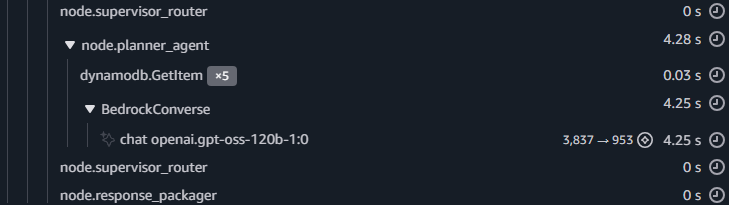
\includegraphics[width=0.95\linewidth,height=0.60\textheight,keepaspectratio]{../assets/images/agentcore_v1_observability/observability_3.png}}
\end{center}


\newpage
\DocNeedspace{8\baselineskip}
\section*{4. 기능 테스트 (Functional)}
\addcontentsline{toc}{section}{4. 기능 테스트 (Functional)}

\DocNeedspace{6\baselineskip}
\subsection*{4.1 요구사항}
\addcontentsline{toc}{subsection}{4.1 요구사항}

"검증 기준"의 따옴표 값은 출력 상태값이다.
\par\noindent(\texttt{ok}=정상 추천, \texttt{insufficient}=후보 부족→축소, \texttt{no\_\allowbreak{}candidate}=추천 불가, 자세한 설명은 4.3절.)

\begin{footnotesize}
\begin{longtable}{@{}L{0.120\linewidth}L{0.160\linewidth}L{0.250\linewidth}L{0.250\linewidth}L{0.145\linewidth}@{}}
\toprule
\TblHead{0.120\linewidth}{ID} & \TblHead{0.160\linewidth}{시나리오} & \TblHead{0.250\linewidth}{검증 기준} & \TblHead{0.250\linewidth}{관련 요구사항} & \TblHead{0.145\linewidth}{대상 케이스} \\
\midrule
\endhead
\bottomrule
\endlastfoot
FN-03 & 도시 발견·추천 정상 & 선택 도시 존재, 추천 장소 3개 이상, 상태 \texttt{ok} & FR-REC-001, FR-RAG-001/002 & 01--03, 05, 06, 08--10, 15, 17, 19--21 \\
FN-04 & 축제 포함 추천 & 축제 후보 수집 + 일정에 배치(또는 정당한 미배치) & FR-FES-001, FR-FEST-ENTRY-001 & 12, 13, 14, 16 \\
FN-05 & 일정 생성 & 일정 생성 + 일정 검증 통과 & FR-TRIP-001\textasciitilde004 & 정상 경로 전체 \\
FN-07 & 단계 라우팅 & 노드 방문 순서 = 설계 그래프 & FR-RAG-002 & 전 케이스 \\
FN-입력추출 & 앱/HTTP 래핑 입력 파싱 & 래핑된 요청 정상 추출 & FR-COM-001 & 15, 16 \\
FB-03 & 추천 불가(내륙 도시+해안 테마) & 상태 \texttt{no\_\allowbreak{}candidate} + 사용자 재질의 & NFR-005 & 22 \\
FB-05 & 후보 부족 → 축소 일정 & 축소 일정 구성, 상태 \texttt{insufficient} & FR-TRIP-002 & 04, 07, 11 \\
FB-검증 & 잘못된 입력 안전 거부 & 입력 거부, 오류 미전파 & NFR-005 & 18 \\
SC-* & 출력 필수 필드 완전성 & 추천·일정·축제 출력의 필수 필드 존재 & FR-REC-003 & 전 케이스 \\
SF-FEST & 미확정 축제 배치 금지 & 날짜 미확정 축제는 일정에 넣지 않음 & FR-FES-001 & 12, 13, 14, 16 \\
\end{longtable}
\end{footnotesize}

\begin{quote}
관련 요구사항은 기능/비기능 요구사항 ID에 \textbf{근사 매핑}한 것이다.
\par\noindent 요구사항 정의가 개략적이라 1:1 대응은 아니며, 매핑은 평가자 참고용이다.
\end{quote}

\newpage
\DocNeedspace{6\baselineskip}
\subsection*{\SubsectionBreak{4.2 결과}{22 케이스 (Path 1, 로컬 e2e dump)}}
\addcontentsline{toc}{subsection}{4.2 결과 / 22 케이스 (Path 1, 로컬 e2e dump)}

\begin{footnotesize}
\begin{longtable}{@{}C{0.043\linewidth}L{0.270\linewidth}C{0.100\linewidth}C{0.120\linewidth}C{0.110\linewidth}C{0.140\linewidth}L{0.115\linewidth}@{}}
\toprule
\TblHead{0.043\linewidth}{\#} & \TblHead{0.270\linewidth}{케이스} & \TblHead{0.100\linewidth}{진입} & \TblHead{0.120\linewidth}{상태} & \TblHead{0.110\linewidth}{응답} & \TblHead{0.140\linewidth}{축제 배치/미배치} & \TblHead{0.115\linewidth}{선택 도시} \\
\midrule
\endhead
\bottomrule
\endlastfoot
01 & coast\_quiet & chat & ok & completed & 0/0 & 삼척시 \\
02 & coast\_vibrant & chat & ok & completed & 0/0 & 강릉시 \\
03 & nature\_quiet & chat & ok & completed & 0/0 & 원주시 \\
04 & nature\_vibrant & chat & insufficient & completed & 0/0 & 원주시 \\
05 & history & chat & ok & completed & 0/0 & 안동시 \\
06 & art & chat & ok & completed & 0/0 & 강릉시 \\
07 & healing & chat & insufficient & completed & 0/0 & 영양군 \\
08 & nature+coast 3d2n & chat & ok & completed & 0/0 & 영덕군 \\
09 & history+nature (서울) & chat & ok & completed & 0/0 & 고령군 \\
10 & coast+healing daytrip (대구) & chat & ok & completed & 0/0 & 양양군 \\
11 & home nature+healing 3d2n (서울) & home\_\allowbreak{}rec & insufficient & completed & 0/0 & 영양군 \\
12 & history + festival & chat & ok & completed & 0/1 & 성주군 \\
13 & sea + festival & chat & ok & completed & 1/0 & 강릉시 \\
14 & map\_\allowbreak{}marker(경주) history + festival & map\_\allowbreak{}marker & ok & completed & 1/0 & 경주시 \\
15 & wrapped(agentcore) history+art & wrap & ok & completed & 0/0 & 강릉시 \\
16 & wrapped(http) nature + festival & wrap & ok & completed & 1/0 & 평창군 \\
17 & rare combo art+healing & chat & ok & completed & 0/0 & 인제군 \\
18 & invalid map\_\allowbreak{}marker (destinationId 누락) & map\_\allowbreak{}marker & -- & END\_\allowbreak{}WAIT\_\allowbreak{}USER & 0/0 & -- (안전 거부) \\
19 & intent short query & chat & ok & completed & 0/0 & 동해시 \\
20 & intent long complex query & chat & ok & completed & 0/0 & 울진군 \\
21 & map\_\allowbreak{}marker(경주) history (no festival) & map\_\allowbreak{}marker & ok & completed & 0/0 & 경주시 \\
22 & no\_\allowbreak{}candidate (내륙 영양 + 해안) & map\_\allowbreak{}marker & no\_\allowbreak{}candidate & END\_\allowbreak{}WAIT\_\allowbreak{}USER & 0/0 & -- (no\_\allowbreak{}city\_\allowbreak{}after\_\allowbreak{}theme\_\allowbreak{}gate) \\
\end{longtable}
\end{footnotesize}

\DocNeedspace{6\baselineskip}
\subsection*{4.3 Fallback / 예외 경로 정리}
\addcontentsline{toc}{subsection}{4.3 Fallback / 예외 경로 정리}

정상(ok) 외 경로를 유형별로 분리한다.
\par\noindent 전부 \textbf{에러가 아니라 설계된 안전 동작}이며 실행 자체는 성공(노드 status=success)이다.

\begin{footnotesize}
\begin{longtable}{@{}L{0.120\linewidth}L{0.160\linewidth}L{0.250\linewidth}L{0.250\linewidth}L{0.145\linewidth}@{}}
\toprule
\TblHead{0.120\linewidth}{유형} & \TblHead{0.160\linewidth}{케이스} & \TblHead{0.250\linewidth}{트리거} & \TblHead{0.250\linewidth}{동작} & \TblHead{0.145\linewidth}{응답} \\
\midrule
\endhead
\bottomrule
\endlastfoot
축소 일정 (insufficient\_\allowbreak{}candidates) & 04, 07, 11 & 도시는 찾았으나 후보 \textless{} 필요 일정 수 & 가능 범위로 축소 일정 + userNotice & completed \\
축제 미배치 (게이트) & 12 & 축제 날짜가 여행기간과 불일치 & 도시 ok, 축제만 미배치(없는 사실 배치 안 함) & completed \\
no\_\allowbreak{}candidate (재질의) & 22 & 테마 게이트 통과 도시 0 & 추천 생성 안 함, 사용자 재질의 요청 & END\_\allowbreak{}WAIT\_\allowbreak{}USER \\
validation 거부 (안전 격리) & 18 & 스키마 위반 입력(destinationId 누락) & intent 단계 조기 거부, LLM 미호출 & END\_\allowbreak{}WAIT\_\allowbreak{}USER \\
\end{longtable}
\end{footnotesize}

세부:

\begin{itemize}
\tightlist
\item
  \textbf{04 / 07 / 11 (축소):} 04 원주 recommended 4 \textless{} 필요 5 · 07 영양 2 \textless{} 5 · 11 영양 6 \textless{} 8.\par\noindent
  모두 userNotice \texttt{"후보\ 수가\ 적어\ 가능한\ 범위에서\ 축소\ 일정을\ 구성했습니다.\allowbreak{}"} 포함, 일정은 정상 생성(각 2·1·2일).
\item
  \textbf{12 (축제 skip):} 성주 ok, festival\_skipped=1.\par\noindent
  미확정 축제를 확정 일정에 끼워넣지 않는 게이트 동작(SF-FEST).
\item
  \textbf{22 (no\_candidate):} failure\_signal=\texttt{no\_\allowbreak{}city\_\allowbreak{}after\_\allowbreak{}theme\_\allowbreak{}gate}, 일정 없음.
\item
  \textbf{18 (거부):} 일정 없음, 토큰 0.\par\noindent
  오류가 다음 단계로 번지지 않음.
\end{itemize}

\DocNeedspace{6\baselineskip}
\subsection*{4.4 단계별 대표 테스트 케이스 (정식 TC)}
\addcontentsline{toc}{subsection}{4.4 단계별 대표 테스트 케이스 (정식 TC)}

각 경로의 대표 케이스를 \textbf{전제 → 입력 → 실행 단계 → 기대 결과 → 실측 결과 → 판정} 양식으로 기술한다.
\par\noindent 실행 단계는 LangGraph 파이프라인 노드 진행을 따른다.

\textbf{TC-14}\par\noindent
\textbf{앵커 + 축제 (핵심 복합 경로)}

\begin{small}
\begin{longtable}{@{}L{0.205\linewidth}L{0.755\linewidth}@{}}
\toprule
\TblHead{0.205\linewidth}{구분} & \TblHead{0.755\linewidth}{내용} \\
\midrule
\endhead
\bottomrule
\endlastfoot
전제 & 데이터에 경주(KR-47-130) 및 2026-10월 신라문화제 적재 / map\_marker 진입 \\
입력 & entryType=map\_marker, destinationId=경주, themes={[}history{]}, tripType=daytrip, includeFestivals=true, travelMonth=10 \\
실행 단계 & ① 의도 분석: 도시 고정(anchored) 모드 확정 → ② 단계 라우팅 → ③ 후보 검색: 경주로 한정한 벡터검색(50개 후보) + 축제 후보 수집 → ④ 축제 검증: 신라문화제 날짜 확정 → ⑤ 일정 구성: 일정 배치 + 축제 삽입 → ⑥ 응답 정리 \\
기대 결과 & status=ok, 선택 도시=경주, 축제 placed=1, 응답 completed \\
실측 결과 & status=\texttt{ok}, 경주시(city\_score 2.9163), recommended 6, 신라문화제(FEST-1718137, 10-09\textasciitilde11) \textbf{placed 1/skip 0}, 1일차 첫 항목=경주역사유적지구, completed \\
판정 & \textbf{Pass}\par\noindent 도시 고정 + 축제 검증·배치가 한 요청에서 동시에 정상 동작 \\
\end{longtable}
\end{small}

\textbf{TC-13}\par\noindent
\textbf{축제 정상 배치 (발견 + 축제)}

\begin{small}
\begin{longtable}{@{}L{0.205\linewidth}L{0.755\linewidth}@{}}
\toprule
\TblHead{0.205\linewidth}{구분} & \TblHead{0.755\linewidth}{내용} \\
\midrule
\endhead
\bottomrule
\endlastfoot
전제 & 해당 월 해안 도시에 축제 적재 \\
입력 & entryType=chat, themes={[}sea\_coast{]}, tripType=2d1n, includeFestivals=true \\
실행 단계 & ① 의도 분석(축제 시드 모드) → ② 축제 보유 도시로 검색 범위 제한 → ③ 도시 선택 → ④ 축제 검증(날짜 확정) → ⑤ 일정에 축제 삽입 \\
기대 결과 & status=ok, 축제 placed=1, 일정 2일 \\
실측 결과 & status=\texttt{ok}, 강릉시(2.7714), recommended 8, 강릉비치비어페스티벌 \textbf{placed 1}, 2일, completed \\
판정 & \textbf{Pass} \\
\end{longtable}
\end{small}

\textbf{TC-05}\par\noindent
\textbf{단일 테마 정상 (발견)}

\begin{small}
\begin{longtable}{@{}L{0.205\linewidth}L{0.755\linewidth}@{}}
\toprule
\TblHead{0.205\linewidth}{구분} & \TblHead{0.755\linewidth}{내용} \\
\midrule
\endhead
\bottomrule
\endlastfoot
전제 & 역사 테마 풍부 도시(안동) 적재 \\
입력 & entryType=chat, themes={[}history{]}, tripType=2d1n, includeFestivals=false \\
실행 단계 & ① 의도 분석(역사 테마 추출) → ② 전역 벡터검색 → ③ 도시 점수화·선택 → ④ 일정 구성 \\
기대 결과 & status=ok, 역사 정합 도시, recommended ≥ 3 \\
실측 결과 & status=\texttt{ok}, 안동시(2.4734), retrieved 50 → recommended 10, 일정 2일 \\
판정 & \textbf{Pass}\par\noindent 단일 역사 테마 → 안동(테마-도시 정합) \\
\end{longtable}
\end{small}

\textbf{TC-22}\par\noindent
\textbf{no\_candidate (열화 경로 / 안정성)}

\begin{small}
\begin{longtable}{@{}L{0.205\linewidth}L{0.755\linewidth}@{}}
\toprule
\TblHead{0.205\linewidth}{구분} & \TblHead{0.755\linewidth}{내용} \\
\midrule
\endhead
\bottomrule
\endlastfoot
전제 & 영양(KR-Yeongyang)은 내륙(해안 없음) / map\_marker 진입 \\
입력 & entryType=map\_marker, destinationId=영양, themes={[}sea\_coast{]}, tripType=daytrip \\
실행 단계 & ① 의도 분석(도시 고정 모드) → ② 후보 검색: 영양 내 해안 관광지 검색 → 테마 조건 통과 도시 0 → 추천 불가 처리 \\
기대 결과 & status=no\_candidate, failure\_signal=no\_city\_after\_theme\_gate, 재질의 \\
실측 결과 & status=\texttt{no\_\allowbreak{}candidate}, failure=\texttt{no\_\allowbreak{}city\_\allowbreak{}after\_\allowbreak{}theme\_\allowbreak{}gate}, needs\_clarification=true, 응답 END\_WAIT\_USER \\
판정 & \textbf{Pass}\par\noindent 불가능 조합을 환각 없이 안전 거부 + 재질의 \\
\end{longtable}
\end{small}

\textbf{TC-18}\par\noindent
\textbf{validation negative (입력 검증 / 안정성)}

\begin{small}
\begin{longtable}{@{}L{0.205\linewidth}L{0.755\linewidth}@{}}
\toprule
\TblHead{0.205\linewidth}{구분} & \TblHead{0.755\linewidth}{내용} \\
\midrule
\endhead
\bottomrule
\endlastfoot
전제 & map\_marker는 destinationId 필수 \\
입력 & entryType=map\_marker, \textbf{destinationId 누락}, themes={[}sea\_coast{]}, tripType=daytrip \\
실행 단계 & ① 의도 분석: 입력 검증 실패 감지 → 조기 거부(LLM 미호출) → ② 단계 라우팅 → ⑥ 응답 정리 \\
기대 결과 & 안전 거부, 에러 미전파, 응답 END\_WAIT\_USER \\
실측 결과 & 거부 처리, 응답 END\_WAIT\_USER, 텔레메트리 \textbf{3노드·토큰 0}(LLM 미호출 조기 거부) \\
판정 & \textbf{Pass}\par\noindent 잘못된 입력이 하류로 전파되지 않고 intent 단계 격리 \\
\end{longtable}
\end{small}

\DocNeedspace{6\baselineskip}
\subsection*{4.5 판정}
\addcontentsline{toc}{subsection}{4.5 판정}

\begin{small}
\begin{longtable}{@{}L{0.205\linewidth}L{0.755\linewidth}@{}}
\toprule
\TblHead{0.205\linewidth}{요구사항} & \TblHead{0.755\linewidth}{결과} \\
\midrule
\endhead
\bottomrule
\endlastfoot
FN-03 도시 발견 & \textbf{Pass}\par\noindent 정상 케이스 전부 status=ok, selected\_city·recommended\_places 존재 \\
FN-04 축제 & \textbf{Pass}\par\noindent 13·14·16 일정 배치(placed=1), 12 정당한 skip(4.3절) \\
FN-07 라우팅 & \textbf{Pass}\par\noindent 축제 검증 노드가 축제 포함 요청(12·13·14·16)에서만 실행, 그 외 미실행 \\
FN-입력추출 & \textbf{Pass}\par\noindent 15(agentcore), 16(http) wrapper 정상 \\
FB-03 no\_candidate & \textbf{Pass}\par\noindent 22: status=no\_candidate, failure\_signal=\texttt{no\_\allowbreak{}city\_\allowbreak{}after\_\allowbreak{}theme\_\allowbreak{}gate} \\
FB-05 insufficient & \textbf{Pass}\par\noindent 04·07·11 status=insufficient, 응답 완료(축소 경로) \\
FB-검증 negative & \textbf{Pass}\par\noindent 18: 안전 거부(END\_WAIT\_USER), 에러 미전파 \\
SC-* 스키마 계약 & \textbf{Pass}\par\noindent 전 케이스 CE 패키지·Planner·축제 필수 필드 완전 \\
SF-FEST 축제 게이트 & \textbf{Pass}\par\noindent 미배치 축제는 모두 게이트 skip, 환각 배치 0 \\
에러율 & \textbf{Pass}\par\noindent 정상 시나리오 status=error 0 \\
\end{longtable}
\end{small}

\textbf{기능 결론: 22/22 Pass.}

\DocNeedspace{6\baselineskip}
\subsection*{\SubsectionBreak{4.6 후속 관찰}{실패 아님 / V2 참고}}
\addcontentsline{toc}{subsection}{4.6 후속 관찰 (실패 아님 / V2 참고)}

\begin{itemize}
\tightlist
\item
  \textbf{12번 축제 0/1 (skip):} 4개 축제 케이스 중 유일하게 미배치.\par\noindent
  게이트에 의한 정당한 skip으로 보이나 date\_status 근거 1건 확인 권장.
\item
  \textbf{17번:} fixture 설계상 기대는 clarify/no\_candidate였으나 실제 ok(인제군).\par\noindent
  해당 조합이 실제로 후보가 존재 → 테스트 플랜의 17 기대값 재조정 필요.
\item
  \textbf{10번:} 대구 출발 daytrip인데 양양군(원거리 강원) 선택.\par\noindent
  거리 가중 동작 점검 대상.
\item
  \textbf{04 vs 03:} nature 테마에서 두 변형이 동일 도시(원주) 선택.
\end{itemize}

\DocNeedspace{6\baselineskip}
\subsection*{\SubsectionBreak{4.7 예시}{e2e dump 원본 (Path 1)}}
\addcontentsline{toc}{subsection}{4.7 예시 / e2e dump 원본 (Path 1)}

\begin{verbatim}
[14번]
정상 + 축제
{
  "status": "ok",
  "selected_city": { "city_id": "KR-47-130", "city_name_ko": "경주시", "city_score": 2.9163 },
  "counts": { "retrieved": 50, "scored": 50, "recommended_places": 6, "required_itinerary_places": 3 },
  "festival": { "festival_id": "FEST-1718137", "name": "신라문화제",
                "event_start_date": "2026-10-09", "event_end_date": "2026-10-11" },
  "festival_validation": { "placed": 1, "skipped": 0 },
  "itinerary_day1_item1": { "title": "경주역사유적지구 [유네스코 세계유산]", "contentId": "attraction#971032" },
  "response_status": "completed"
}

[22번]
no_candidate
{
  "status": "no_candidate",
  "failure_signals": ["no_city_after_theme_gate"],
  "needs_clarification": true,
  "response_status": "END_WAIT_USER"
}
\end{verbatim}


\newpage
\DocNeedspace{8\baselineskip}
\section*{5. 비기능 테스트 (Non-Functional)}
\addcontentsline{toc}{section}{5. 비기능 테스트 (Non-Functional)}

\DocNeedspace{6\baselineskip}
\subsection*{5.1 요구사항}
\addcontentsline{toc}{subsection}{5.1 요구사항}

\begin{footnotesize}
\begin{longtable}{@{}L{0.135\linewidth}L{0.215\linewidth}L{0.265\linewidth}L{0.325\linewidth}@{}}
\toprule
\TblHead{0.135\linewidth}{ID} & \TblHead{0.215\linewidth}{측정} & \TblHead{0.265\linewidth}{검증 기준} & \TblHead{0.325\linewidth}{관련 요구사항} \\
\midrule
\endhead
\bottomrule
\endlastfoot
NF-LAT-svc & 벡터검색·DB 콜 지연 & 데이터 서비스 콜이 \textbf{1초 내} 완료 & NFR-001C (벡터검색 1초 이내) \\
NF-LAT-ceil & 전체 요청 응답시간 & 기준값 기록 (요구사항 8초와 대조) & NFR-001B (에이전트 8초 이내) \\
NF-TOKEN & 요청당 토큰 사용량 & 노드별·요청당 토큰 기록 & 해당 없음 \\
OB-01 & 노드 메트릭 로그 스키마 & 요청ID·노드명·소요시간·상태·토큰 필드 존재 & NFR(관측) \\
OB-에러 & 에러율 & 정상 시나리오에서 오류 0 & NFR(안정성) \\
\end{longtable}
\end{footnotesize}

수집: 배포 런타임 22 케이스 호출 → X-Ray 트레이스 + CloudWatch 노드 메트릭 로그.
\par\noindent 헬스체크(\texttt{/\allowbreak{}ping}) 스팬은 집계에서 제외.

\begin{quote}
\textbf{집계 대상 명확화:} 22 호출 \textbf{전부 실행 성공}(노드 status=success, X-Ray fault 0)이라 "성공분만 골라 잰" 게 아니라 \textbf{실패한 콜이 0개}여서 제외할 것이 없었다.
\par\noindent fallback 케이스(04·07·11 insufficient, 22 no\_candidate, 18 reject)도 실행 성공이므로 그 콜이 모두 집계에 포함된다.
\par\noindent 단 \textbf{18번(validation 거부)은 검색 이전 intent 단계에서 거부}돼 S3Vectors/Dynamo\allowbreak{}DB를 호출하지 않았다.
\par\noindent 즉 필터링이 아니라 호출 자체가 없어서 서비스-콜 보유 트레이스는 21개다.
\end{quote}

\DocNeedspace{6\baselineskip}
\subsection*{\SubsectionBreak{5.2 결과}{서비스 콜 지연 (X-Ray, 22 케이스 전수)}}
\addcontentsline{toc}{subsection}{5.2 결과 / 서비스 콜 지연 (X-Ray, 22 케이스 전수)}

X-Ray 하위 구간 소요시간(네트워크 포함 실제 왕복).
\par\noindent 평균 포함, 단위 = 초.

\begin{footnotesize}
\begin{longtable}{@{}L{0.200\linewidth}L{0.082\linewidth}L{0.102\linewidth}L{0.102\linewidth}L{0.122\linewidth}L{0.122\linewidth}L{0.165\linewidth}@{}}
\toprule
\TblHead{0.200\linewidth}{서비스} & \TblHead{0.082\linewidth}{콜 수} & \TblHead{0.102\linewidth}{mean} & \TblHead{0.102\linewidth}{min} & \TblHead{0.122\linewidth}{median} & \TblHead{0.122\linewidth}{p90} & \TblHead{0.165\linewidth}{max} \\
\midrule
\endhead
\bottomrule
\endlastfoot
\textbf{Dynamo\allowbreak{}DB} & 118 & \textbf{0.011} & 0.003 & 0.005 & 0.038 & \textbf{0.058} \\
\textbf{S3Vectors} & 56 & \textbf{0.092} & 0.064 & 0.089 & 0.119 & \textbf{0.127} \\
Bedrock\allowbreak{}Runtime (LLM) & 100 & \textbf{2.906} & 0.079 & 1.604 & 8.514 & 15.719 \\
\end{longtable}
\end{footnotesize}

\textbf{판정 (NF-LAT-svc): Pass.}
\par\noindent Dynamo\allowbreak{}DB 평균 11ms·최악 58ms, S3Vectors 평균 92ms·최악 127ms.
\par\noindent 단 한 콜도 1초를 넘지 않는다(목표 압도적 충족).
\par\noindent 검색·DB는 무시할 수준이고, 요청 시간은 \textbf{사실상 전부 LLM(Bedrock\allowbreak{}Runtime, 평균 2.9초/콜)} 이 차지한다.
\par\noindent → 최적화 대상은 검색/DB가 아니라 LLM 호출(특히 일정 설명 생성).

\DocNeedspace{6\baselineskip}
\subsection*{\SubsectionBreak{5.3 결과}{전체 요청 응답시간 (22 케이스)}}
\addcontentsline{toc}{subsection}{5.3 결과 / 전체 요청 응답시간 (22 케이스)}

\begin{small}
\begin{longtable}{@{}L{0.205\linewidth}L{0.755\linewidth}@{}}
\toprule
\TblHead{0.205\linewidth}{지표} & \TblHead{0.755\linewidth}{값} \\
\midrule
\endhead
\bottomrule
\endlastfoot
평균 & 13.8s \\
중앙값 & 15.7s \\
최대 & 20.4s \\
\end{longtable}
\end{small}

\textbf{요구사항 NFR-001B(에이전트 8초 이내) 대조.}\quad 본 측정은 \textbf{호출마다 새 세션 = 콜드 인스턴스}(요청 간 격리) 조건이라 중앙값 15.7s로 \textbf{8초 목표를 초과}한다.
\par\noindent 초과분은 거의 전부 LLM 생성 시간(특히 일정 설명 생성)이며 검색·DB는 5.2절 기준 1초 미만이다.
\par\noindent 즉 \textbf{벡터검색 요구(NFR-001C 1초)는 충족, 전체 응답 요구(NFR-001B 8초)는 콜드 기준 미달}이다.
\par\noindent 워밍 인스턴스 재사용 시 단축 여지가 있으나 본 라운드 미측정이다.
\par\noindent LLM 호출 최적화가 9장에서 정리한 8초 목표 달성의 핵심 과제다.

\DocNeedspace{6\baselineskip}
\subsection*{\SubsectionBreak{5.4 결과}{\texorpdfstring{노드/토큰 (CloudWatch \texttt{AGENT\_\allowbreak{}NODE\_\allowbreak{}METRIC}, 22 케이스)}{노드/토큰 (CloudWatch AGENT\_NODE\_METRIC, 22 케이스)}}}
\addcontentsline{toc}{subsection}{5.4 결과 / 노드·토큰 (CloudWatch AGENT\_NODE\_METRIC, 22 케이스)}

요청당 노드 실행 수·토큰 합 (발췌, 전 케이스 실패 0).

\begin{footnotesize}
\begin{longtable}{@{}L{0.275\linewidth}L{0.120\linewidth}L{0.082\linewidth}L{0.215\linewidth}L{0.230\linewidth}@{}}
\toprule
\TblHead{0.275\linewidth}{case} & \TblHead{0.120\linewidth}{노드 수} & \TblHead{0.082\linewidth}{실패} & \TblHead{0.215\linewidth}{축제 검증} & \TblHead{0.230\linewidth}{토큰 합} \\
\midrule
\endhead
\bottomrule
\endlastfoot
01 coast\_quiet & 7 & 0 & -- & 8,131 \\
05 history & 7 & 0 & -- & 9,051 \\
14 anchor+festival & 9 & 0 & \checkmark{} & 7,299 \\
16 wrap+festival & 9 & 0 & \checkmark{} & 7,564 \\
18 invalid & 3 & 0 & -- & 0 \\
20 long query & 7 & 0 & -- & 9,415 \\
22 no\_candidate & 5 & 0 & -- & 2,038 \\
\end{longtable}
\end{footnotesize}

관측: 토큰 2,038(22, 축소)--9,415(20, 긴 쿼리).
\par\noindent \textbf{18(입력 거부)은 토큰 0}.
\par\noindent LLM 미호출 조기 거부.
\par\noindent \textbf{22(추천 불가)는 5노드로 축소.}
\par\noindent 축제 케이스(12·13·14·16)만 9노드(축제 검증 포함) → 라우팅 정확성의 텔레메트리 증거.

\DocNeedspace{6\baselineskip}
\subsection*{\SubsectionBreak{5.5 결과}{운영/관측}}
\addcontentsline{toc}{subsection}{5.5 결과 / 운영·관측}

\begin{small}
\begin{longtable}{@{}L{0.205\linewidth}L{0.755\linewidth}@{}}
\toprule
\TblHead{0.205\linewidth}{항목} & \TblHead{0.755\linewidth}{결과} \\
\midrule
\endhead
\bottomrule
\endlastfoot
HTTP 200 & 22/22 (invoke 응답) \\
X-Ray \texttt{hasError} & 전 케이스 트레이스 false (오류 0) \\
노드 status & 전 케이스 전 노드 \texttt{success} (fail 0) \\
OB-01 스키마 & \texttt{AGENT\_\allowbreak{}NODE\_\allowbreak{}METRIC} requestId·nodeName·durationMs·status·llmMetrics 전부 존재 \\
\texttt{/\allowbreak{}ping} 분리 & 집계에서 정상 제외 \\
\end{longtable}
\end{small}

\textbf{판정 (OB-에러): Pass.}
\par\noindent 22 케이스 invoke 전수에서 fault·node error 0.

\DocNeedspace{6\baselineskip}
\subsection*{\SubsectionBreak{5.6 예시}{X-Ray trace 원본 (Path 2)}}
\addcontentsline{toc}{subsection}{5.6 예시 / X-Ray trace 원본 (Path 2)}

단일 요청의 segment 분해 (trace \texttt{1-\allowbreak{}6a403501-\allowbreak{}.\allowbreak{}.\allowbreak{}.\allowbreak{}}, 총 17.997s, 단위 초).
\par\noindent 콘솔 타임라인은 3.2절 {[}화면 2·3{]}을 참조한다(별도 샘플 트레이스, 총 11.11s).

\begin{verbatim}
LovvAgentCore_LovvAgentV1.DEFAULT   17.997   (root / 요청 전체)
  BedrockRuntime                                  9.982   ← LLM
  BedrockRuntime                                  6.234   ← LLM
  BedrockRuntime                                  1.116   ← LLM
  S3Vectors                          0.115
  BedrockRuntime                                  0.105
  BedrockRuntime                                  0.083
  S3Vectors                          0.070
  DynamoDB                            0.041
  DynamoDB                            0.005
  DynamoDB                            0.004
  DynamoDB                            0.004
  DynamoDB                            0.004
\end{verbatim}

→ 전체 시간의 거의 100\%가 Bedrock\allowbreak{}Runtime(LLM).
\par\noindent S3Vectors·Dynamo\allowbreak{}DB는 합쳐도 0.4초 미만.

\texttt{AGENT\_\allowbreak{}NODE\_\allowbreak{}METRIC} 로그 1건 (노드 메트릭 스키마):

\begin{verbatim}
{"requestId":"REQ-TC-01","logType":"AGENT_NODE_METRIC","nodeName":"intent_agent",
 "durationMs":2502,"status":"success",
 "inputSummary":{"themes":["sea_coast"],"tripType":"2d1n","includeFestivals":false,"queryLength":60},
 "llmMetrics":{"modelId":"openai.gpt-oss-120b-1:0","inputTokens":1814,"outputTokens":254,
               "totalTokens":2068,"contextUsagePercent":1.034}}
\end{verbatim}


\newpage
\DocNeedspace{8\baselineskip}
\section*{6. 모델링 평가 결과 (동작·관측 기반)}
\addcontentsline{toc}{section}{6. 모델링 평가 결과 (동작·관측 기반)}

LovvAgentV1은 학습된 단일 모델이 아니라 \textbf{LLM(gpt-oss-120b) + 임베딩(titan) + 결정론 로직}의 합성 파이프라인이다.
\par\noindent 따라서 "모델링 평가"는 추천 품질의 정답 비교가 아니라, \textbf{각 모델 구성요소의 동작·관측 지표}로 수행한다(품질 oracle 평가는 8장 한계 참조, V2 과제).

\DocNeedspace{6\baselineskip}
\subsection*{6.1 구성요소별 동작 평가}
\addcontentsline{toc}{subsection}{6.1 구성요소별 동작 평가}

\begin{footnotesize}
\begin{longtable}{@{}L{0.135\linewidth}L{0.215\linewidth}L{0.265\linewidth}L{0.325\linewidth}@{}}
\toprule
\TblHead{0.135\linewidth}{구성요소} & \TblHead{0.215\linewidth}{평가 지표} & \TblHead{0.265\linewidth}{실측 (22 케이스)} & \TblHead{0.325\linewidth}{판정} \\
\midrule
\endhead
\bottomrule
\endlastfoot
\textbf{의도 분석 LLM} & 실행 모드 결정·테마 추출·분위기 신호 & 진입별 모드 정확(도시 고정/발견/축제), 분위기 없으면 빈 값(지어내지 않음) & 정상 \\
\textbf{Embedding (titan)} & 테마별 임베딩 호출 & 테마당 ×2(raw+soft), 검색 입력 정상 & 정상 \\
\textbf{검색 (S3Vectors)} & retrieved 후보 수 & 테마당 50 retrieved, 도시 스코어링 입력 & 정상 \\
\textbf{도시 스코어링·선택} & 상태·선택 도시 & 정상 추천 17 / 축소 3 / 추천 불가 1 / 입력 거부 1, 선택 도시 모두 강원·경북 & 정상 \\
\textbf{축제 검증} & 날짜 검증·배치 정책 & 12·13·14·16에서만 실행, 날짜 확정 축제만 배치, 미확정은 제외 & 정상 \\
\textbf{일정 생성(Planner LLM)} & 일정·설명 생성 & 일정 생성 완료, 설명 텍스트 생성(요청당 최대 \textasciitilde9.4k 토큰) & 정상 \\
\end{longtable}
\end{footnotesize}

\textbf{혼잡도 반영.}
\par\noindent 혼잡도 신호에 따라 선택 도시가 달라진다.
\par\noindent 같은 해안 테마라도 "조용한"(케이스 01)은 한적한 삼척, "활기찬"(케이스 02)은 붐비는 강릉이 선택된다.

\DocNeedspace{6\baselineskip}
\subsection*{6.2 라우팅·안정성 평가}
\addcontentsline{toc}{subsection}{6.2 라우팅·안정성 평가}

\begin{itemize}
\tightlist
\item
  \textbf{라우팅 정확성:} 축제 검증 노드가 축제 포함 요청(12·13·14·16)에서만 실행(9노드), 그 외 7노드.\par\noindent
  18(검증 거부)=3노드·토큰 0, 22(추천 불가)=5노드 축소.\par\noindent
  입력 유형별 분기가 텔레메트리로 정확히 확인됨.
\item
  \textbf{결정론 비중(재현성):} 도시 선택·일정 배치·라우팅은 전부 결정론이고 LLM은 (intent 신호 / 추천 근거 / planner 카피) 3군데로 제한 → 동일 입력 재현성·안정성 확보.
\item
  \textbf{안정성:} 22 케이스 전 노드 정상(success), 오류 0, HTTP 200 22/22.\par\noindent
  비정상·불가 입력(18·22)도 멈춤 없이 안전 거부.\par\noindent
  예외 4종(축소·축제 미배치·추천 불가·검증 거부)을 단계적으로 열화 처리.
\item
  \textbf{자원 여유:} context usage \textless2\% (예: intent 1.034\%), 토큰 요청당 2,038\textasciitilde9,415.\par\noindent
  컨텍스트 한도 대비 충분한 여유.
\end{itemize}

\DocNeedspace{6\baselineskip}
\subsection*{\SubsectionBreak{6.3 추천 충실도}{테마 커버리지 \& 일정 충족}}
\addcontentsline{toc}{subsection}{6.3 추천 충실도 / 테마 커버리지 \& 일정 충족}

테스트 케이스 입력으로 직접 측정 가능한 두 지표로 추천 충실도를 평가한다.

\DocNeedspace{8\baselineskip}
\subsubsection*{6.3.1 테마 커버리지}
\addcontentsline{toc}{subsubsection}{6.3.1 테마 커버리지}

선택 도시가 요청 테마를 모두 포함하는가.

추천이 생성된 20개 케이스 \textbf{전부에서 선택 도시의 테마 커버리지 = 1.0}이다.
\par\noindent 즉 사용자가 고른 모든 테마에 대해 그 도시에 장소가 존재한다.
\par\noindent 다중 테마도 100\%다: 3테마(20번 자연+해안+역사) 선택 도시 울진 1.0, 2테마(10번 해안+힐링) 양양 1.0.
\par\noindent 다중 테마의 테마 균형(엔트로피) 점수도 0.92\textasciitilde0.94로 높아 한 테마에 쏠리지 않는다.

\begin{itemize}
\tightlist
\item
  부분 커버리지 도시(예: 20번 영덕 3분의 2, 10번 경주 2분의 1)는 순위엔 오르지만 \textbf{선택되지 않는다} → 선택 도시는 항상 완전 커버리지.
\item
  한계: 이 지표는 \textbf{도시 단위}(그 도시가 모든 테마의 장소를 보유) 측정이다.
  최종 일정의 각 슬롯까지 테마가 1:1로 분배되는지는 후보 선택의 테마 쿼터에 따르며, 본 지표는 도시 단위까지 보증한다.
\end{itemize}

\DocNeedspace{10\baselineskip}
\subsubsection*{6.3.2 일정 충족}
\addcontentsline{toc}{subsubsection}{6.3.2 일정 충족}

필요한 일정 칸을 채웠는가.

\begin{small}
\begin{longtable}{@{}L{0.195\linewidth}L{0.355\linewidth}L{0.405\linewidth}@{}}
\toprule
\TblHead{0.195\linewidth}{결과} & \TblHead{0.355\linewidth}{케이스 수} & \TblHead{0.405\linewidth}{비율} \\
\midrule
\endhead
\bottomrule
\endlastfoot
충족 (정상 일정) & 17 & 일정 생성 20건 중 \textbf{85\%} \\
부족 (축소 일정) & 3 (04·07·11) & \textbf{15\%} \\
추천 불가·거부 (일정 없음) & 2 (18·22) & 해당 없음 \\
\end{longtable}
\end{small}

\textbf{도시 선택 규칙과 축소 발생 비율.}
\par\noindent 선택 로직은 \textbf{일정을 채울 수 있는 가장 높은 순위의 도시}를 고른다.
\par\noindent 1위가 부족하면 2위·3위를 순차로 시도하고, \textbf{어느 도시도 못 채울 때만} 1위를 그대로 두고 축소 일정을 만든다(\texttt{selection\_\allowbreak{}reason\_\allowbreak{}code}로 확인).

\begin{itemize}
\tightlist
\item
  도시를 탐색한 18개 케이스(지도 마커로 고정한 14·21 제외)에서 \textbf{선택된 도시는 전부 점수 1위}였다.\par\noindent
  17건은 1위가 일정을 채워 정상, 3건(04·07·11, 16.7\%)은 \textbf{모든 후보 도시가 미충족}이라 1위 강제 + 축소(\texttt{city\_\allowbreak{}score\_\allowbreak{}rank\_\allowbreak{}1} + \texttt{insufficient\_\allowbreak{}candidates}).
\item
  즉 "1위는 부족한데 하위 도시는 충분"해서 차순위로 갈아타는 경우는 22개 케이스에서 \textbf{발생하지 않았다}(차순위 선택 로직 자체는 존재하나 이번 입력셋에선 트리거되지 않음).
\item
  도시 고정(앵커) 케이스(14·21)는 순위 선택을 거치지 않으며 둘 다 충족.
\end{itemize}

\DocNeedspace{8\baselineskip}
\textbf{한계(중요).}
\par\noindent \textbf{모든 후보 도시가 일정을 못 채우면}(3건이 이 경우) V1은 축소 일정을 보여주는 것 외의 대안이 없다.
\par\noindent 부족분을 대체 장소로 보충하는 경로가 없어, 가능한 범위로 일정을 줄이고 "후보 수가 적어 축소 일정을 구성했습니다" 안내만 제공한다.
\par\noindent 데이터 풀이 강원·경북 소도시로 한정돼 일부 테마·기간 조합에서 어느 도시도 후보가 얕은 것이 근본 원인이다.

\DocNeedspace{6\baselineskip}
\subsection*{6.4 모델링 평가 종합}
\addcontentsline{toc}{subsection}{6.4 모델링 평가 종합}

동작·관측 관점에서 \textbf{모델 구성요소 전부 정상 거동}하고(intent·검색·스코어링·축제 검증·일정 생성), 라우팅은 입력 유형별로 정확하며, 22 케이스 무에러로 안정적이다.
\par\noindent 충실도 면에서 \textbf{선택 도시는 요청 테마를 100\% 포함}하고, \textbf{일정의 85\%가 정상 충족}된다.
\par\noindent 남은 약점은 후보가 부족할 때 축소 일정 외 대안이 없다는 점이다(6.3절 및 8장).


\newpage
\DocNeedspace{8\baselineskip}
\section*{7. 종합 판정}
\addcontentsline{toc}{section}{7. 종합 판정}

\begin{small}
\begin{longtable}{@{}L{0.195\linewidth}L{0.355\linewidth}L{0.405\linewidth}@{}}
\toprule
\TblHead{0.195\linewidth}{영역} & \TblHead{0.355\linewidth}{케이스} & \TblHead{0.405\linewidth}{결과} \\
\midrule
\endhead
\bottomrule
\endlastfoot
기능 & 22 & \textbf{22/22 Pass} \\
비기능\par\noindent 벡터검색·DB 지연 (NFR-001C) & 22 & \textbf{Pass} (전 콜 1초 미만) \\
비기능\par\noindent 전체 응답시간 (NFR-001B 8초) & 22 & \textbf{미달} (콜드 기준 중앙값 15.7s, 원인=LLM 생성) \\
비기능\par\noindent 운영·관측·안정성 & 22 & \textbf{Pass} (오류 0, 노드 전부 성공, 메트릭 완전) \\
\end{longtable}
\end{small}

\textbf{기능은 22/22 통과}, 안정성도 무에러다(정상·축제·앵커·추천불가·입력거부·축소 일정 경로 모두 설계대로).
\par\noindent 비기능은 \textbf{벡터검색·DB 지연(1초 요구)은 압도적 충족하나, 전체 응답시간 8초 요구는 콜드 인스턴스 기준 미달}(15.7s)이다.
\par\noindent 초과분은 LLM 생성 시간이며 워밍 재사용·LLM 최적화가 9장의 후속 과제다.


\newpage
\DocNeedspace{8\baselineskip}
\section*{8. 한계 / V2 참고}
\addcontentsline{toc}{section}{8. 한계 / V2 참고}

\DocNeedspace{6\baselineskip}
\subsection*{8.1 요구사항 대비 미구현 기능 (제품 문서엔 있으나 V1 에이전트 미구현)}
\addcontentsline{toc}{subsection}{8.1 요구사항 대비 미구현 기능 (제품 문서엔 있으나 V1 에이전트 미구현)}

제품 요구사항에 명시됐으나 V1 추천 에이전트가 \textbf{아직 구현하지 않은} 기능이다.
\par\noindent 평가 시 "범위 외"임을 명확히 한다.

\begin{small}
\begin{longtable}{@{}L{0.195\linewidth}L{0.355\linewidth}L{0.405\linewidth}@{}}
\toprule
\TblHead{0.195\linewidth}{미구현 기능} & \TblHead{0.355\linewidth}{관련 요구사항} & \TblHead{0.405\linewidth}{설명} \\
\midrule
\endhead
\bottomrule
\endlastfoot
\textbf{대체(대안) 일정 추천} & FR-REC-002 & 수집된 월별 날씨 경향을 활용한 대체 일정(우천 대비 등) 미제공 / 단일 일정만 생성 \\
\textbf{우천 대체 일정 팝업} & FR-ENTRY-WEATHER-003 & 폭우·폭설 경향 시 실내형 대체 일정 제안 팝업 없음 \\
\textbf{"추천 다시 받기"} & FR-REC-006 & 직전과 다른 후보로 재추천하는 기능 없음 \\
\textbf{추천 후 후속 질문(멀티턴)} & FR-RAG-003 & 단일 요청만 처리 / 대화 맥락·후속 Q\&A 미지원 \\
\textbf{이동 동선 최적화} & FR-MAP-009 & 일정을 후보 순서대로 배치, 장소 간 이동거리·시간 최적화 안 함 \\
\textbf{미식 식당 추천} & FR-API(미식) & 식당명을 생성하지 않고 외부 검색 링크만 제공 \\
\textbf{숙소 직접 추천} & FR-STAY & 가격·유형 기반 추천 없이 예약 사이트 링크만 \\
\end{longtable}
\end{small}

\DocNeedspace{6\baselineskip}
\subsection*{8.2 테스트·평가상 한계}
\addcontentsline{toc}{subsection}{8.2 테스트·평가상 한계}

\begin{itemize}
\tightlist
\item
  \textbf{데이터 범위:} 적재 데이터가 강원·경북뿐이라 다른 지역은 추천 불가.
\item
  \textbf{추천 충실도는 측정, 절대 품질은 미평가:} 테마 커버리지·일정 충족(6.3절)은 측정했으나, "여러 후보 중 어느 도시가 더 적합한가"의 절대 비교는 별도 평가셋이 필요하다(V2).
\item
  \textbf{추천 내용은 로컬 경로로만 검증:} 배포 텔레메트리(트레이스/로그)에는 추천 내용(선택 도시·축제 배치)이 담기지 않아, 기능 검증은 로컬 실행 결과(Path 1)에 의존한다.
\item
  \textbf{응답시간은 콜드 인스턴스 기준:} 5.3절은 요청마다 새 인스턴스 조건이다.
  워밍 재사용 응답시간은 별도 측정 필요.
\item
  \textbf{장애 주입 미수행:} LLM 실패·재시도 소진 같은 장애 경로는 입력만으로 재현 불가 → 별도 라운드.
\item
  \textbf{후속 관찰 4건(4.6절):} 12 축제 미배치 근거, 17 기대값 재조정, 10 거리 가중, 04 자연 테마 변형.\par\noindent
  비블로커, V2 점검 항목.
\end{itemize}


\newpage
\DocNeedspace{8\baselineskip}
\section*{9. 트레이스 기반 성능 한계 \& V2 보완 지점}
\addcontentsline{toc}{section}{9. 트레이스 기반 성능 한계 \& V2 보완 지점}

X-Ray 트레이스 타임라인에서 드러난 구조적 한계를 정리한다.
\par\noindent 본 섹션은 V2 설계 시 우선순위 참고용이다.

\DocNeedspace{6\baselineskip}
\subsection*{\texorpdfstring{9.1 근거\\[-0.10em]{\normalsize 단일 요청 타임라인 (trace \texttt{1-\allowbreak{}6a403633}, 약 3테마)}}{9.1 근거 단일 요청 타임라인 (trace 1-6a403633, 약 3테마)}}
\addcontentsline{toc}{subsection}{9.1 근거 / 단일 요청 타임라인 (trace 1-6a403633, 약 3테마)}

서비스 콜의 start/end를 시간순으로 나열하면 \textbf{거의 모든 구간이 직렬}이다(단위 ms):

\begin{verbatim}
BedrockRuntime          1799    intent / structured (직렬)
BedrockRuntime            97
BedrockRuntime            91
S3Vectors        102    테마별 검색 6콜: 전부 연속, 겹침 0
S3Vectors        101    (raw+soft × 테마수)  합 약 543ms
S3Vectors        109
S3Vectors         72
S3Vectors         75
S3Vectors         84
DynamoDB          41    visitor stats
BedrockRuntime  6902    ← 일정 설명 생성 (단일 최대 병목)
DynamoDB         4~7    재조회: 장소별 개별 GetItem 8콜 (N+1), 각 4~7ms, 직렬
BedrockRuntime  3883    ← 추가 LLM
\end{verbatim}

비중: LLM \ensuremath{\approx} 12.7s (\textbf{\textasciitilde95\%}) · S3Vectors \ensuremath{\approx} 0.54s · Dynamo\allowbreak{}DB \ensuremath{\approx} 0.08s.
\par\noindent → \textbf{전체 시간의 거의 전부가 LLM이고, 검색+DB는 합쳐 5\% 미만.}

\DocNeedspace{6\baselineskip}
\subsection*{9.2 한계 → V2 보완}
\addcontentsline{toc}{subsection}{9.2 한계 → V2 보완}

\begin{footnotesize}
\begin{longtable}{@{}L{0.120\linewidth}L{0.160\linewidth}L{0.250\linewidth}L{0.250\linewidth}L{0.145\linewidth}@{}}
\toprule
\TblHead{0.120\linewidth}{ID} & \TblHead{0.160\linewidth}{한계} & \TblHead{0.250\linewidth}{트레이스 근거} & \TblHead{0.250\linewidth}{영향} & \TblHead{0.145\linewidth}{V2 보완 방향} \\
\midrule
\endhead
\bottomrule
\endlastfoot
\textbf{L1} & 테마별 S3Vectors \textbf{직렬 호출} (raw+soft × 테마수) & 6콜 연속, 겹침 0, 합 \textasciitilde543ms & 테마 수에 비례해 선형 증가 & 검색 \textbf{병렬화} → 최장 1콜(\textasciitilde100ms)로 수렴, 다테마에서 수백 ms 절감 \\
\textbf{L2} & Dynamo\allowbreak{}DB 재조회 \textbf{N+1} & 장소별 개별 GetItem 8콜 직렬 & 호출 수·비용 증가(추천 장소 수에 비례) & \textbf{BatchGetItem 1콜}로 통합 → 호출 수↓, 비용↓ \\
\textbf{L3} & LLM \textbf{직렬 파이프라인 + 일정 설명 생성 단일 병목} & 일정 설명 LLM 6.9s(전체의 \textasciitilde52\%), LLM 합 \textasciitilde95\% & 요청 응답시간의 사실상 전부 & 모델 경량화/스트리밍, 일정 \textbf{병렬 생성}, 설명 결과 캐싱\par\noindent \textbf{응답시간 최적화의 핵심 타겟} \\
\textbf{L4} & 노드 \textbf{직렬 의존} (의도→후보→일정) & 각 단계가 이전 출력 대기 & 본질적 직렬 & 검색-무관 준비작업 선행 등 부분 파이프라이닝 여지 \\
\end{longtable}
\end{footnotesize}

\DocNeedspace{6\baselineskip}
\subsection*{9.3 V2 우선순위 (트레이스가 말하는 것)}
\addcontentsline{toc}{subsection}{9.3 V2 우선순위 (트레이스가 말하는 것)}

검색/DB(L1·L2)는 \textbf{싸지만 작은} 개선이다(합 0.6s).
\par\noindent \textbf{응답시간의 95\%는 LLM(L3)} 이므로, V2 성능 작업은 L3(특히 일정 설명 생성)에 우선 투자해야 한다.
\par\noindent L1·L2는 다테마·다장소에서 누적되는 비용·확장성 관점에서 의미가 있으나, 단건 응답시간 단축 효과는 제한적이다.
\par\noindent 따라서 V2의 본질적 과제는 \textbf{"검색을 빠르게"가 아니라 "LLM 호출을 줄이거나 병렬화"}하는 것이다.


\newpage
\section*{변경 이력}
\addcontentsline{toc}{section}{변경 이력}
\begin{small}
\begin{longtable}{@{}C{0.135\linewidth}C{0.185\linewidth}C{0.245\linewidth}L{0.375\linewidth}@{}}
\toprule
\TblHead{0.135\linewidth}{버전} & \TblHead{0.185\linewidth}{날짜} & \TblHead{0.245\linewidth}{작성자} & \TblHead{0.375\linewidth}{변경 내용} \\
\midrule
\endhead
v1.0 & 2026-06-28 & 이창우 & LovvAgentV1 테스트 결과 보고서 TeX/PDF 초판 생성 \\
\bottomrule
\end{longtable}
\end{small}


\end{document}
